
% Página 1
\begin{frame}
    \frametitle{Anexo 1}
    \framesubtitle{Limitaciones: EPS}
    \begin{itemize}
        \small
        \item Recursos financieros: Se recurrió a software libre debido al alto costo de las licencias de software de pago.
        \item Tiempo: El proyecto estaba programado para desarrollarse en un periodo limitado de aproximadamente 16 semanas.
        \item Pruebas en laboratorio: La ausencia de equipo especializado, en particular una cámara de vacío térmico, limitó la realización de pruebas experimentales.
        \item Simulaciones: El uso del modelo GFS y el estándar atmosférico ISA, aunque valiosos, tienen limitaciones que pueden afectar la precisión de los resultados.
    \end{itemize}
\end{frame}


% Página 2
\begin{frame}
    \frametitle{Anexo 2}
    \framesubtitle{Antecedentes: EPS}
    \begin{figure}
        \centering
        \begin{minipage}{.5\textwidth}
            \centering
            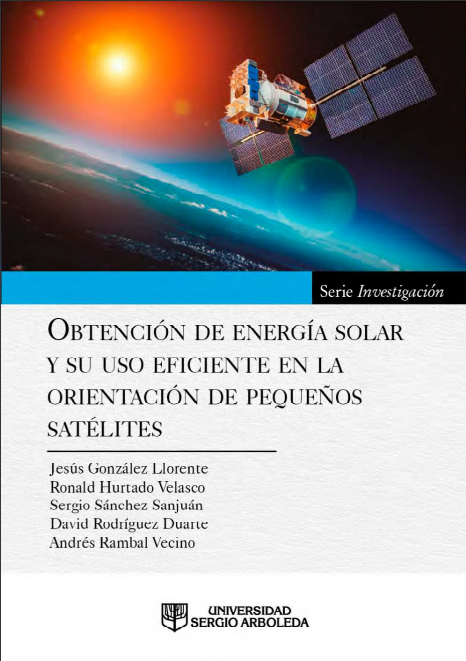
\includegraphics[width=0.38\textheight]{LibroEnergiaSatelites.png} % Reemplaza con tu primera imagen
            \mycaption{Libro ''Obtención de Energía Solar y su Uso Eficiente en la Orientación de Pequeños Satélites'' \cite{energiasat1}}
            \label{fig:sat1}
        \end{minipage}\hfill
        \begin{minipage}{.5\textwidth}
            \centering
            
\includegraphics[width=0.65\textheight]{Birds_logo.png} % Reemplaza con tu segunda imagen
            \vspace*{0.25 cm}
            \mycaption{Proyecto Birds del Kyushu Institute of Technology \cite{jara2022orbit}}
            \label{fig:sat2}
        \end{minipage}
    \end{figure}
    \end{frame}

% Página 3

\begin{frame}
    \frametitle{Anexo 2}
    \framesubtitle{Antecedentes: EPS}
    \begin{figure}
        \centering
        \begin{minipage}{.5\textwidth}
            \centering
            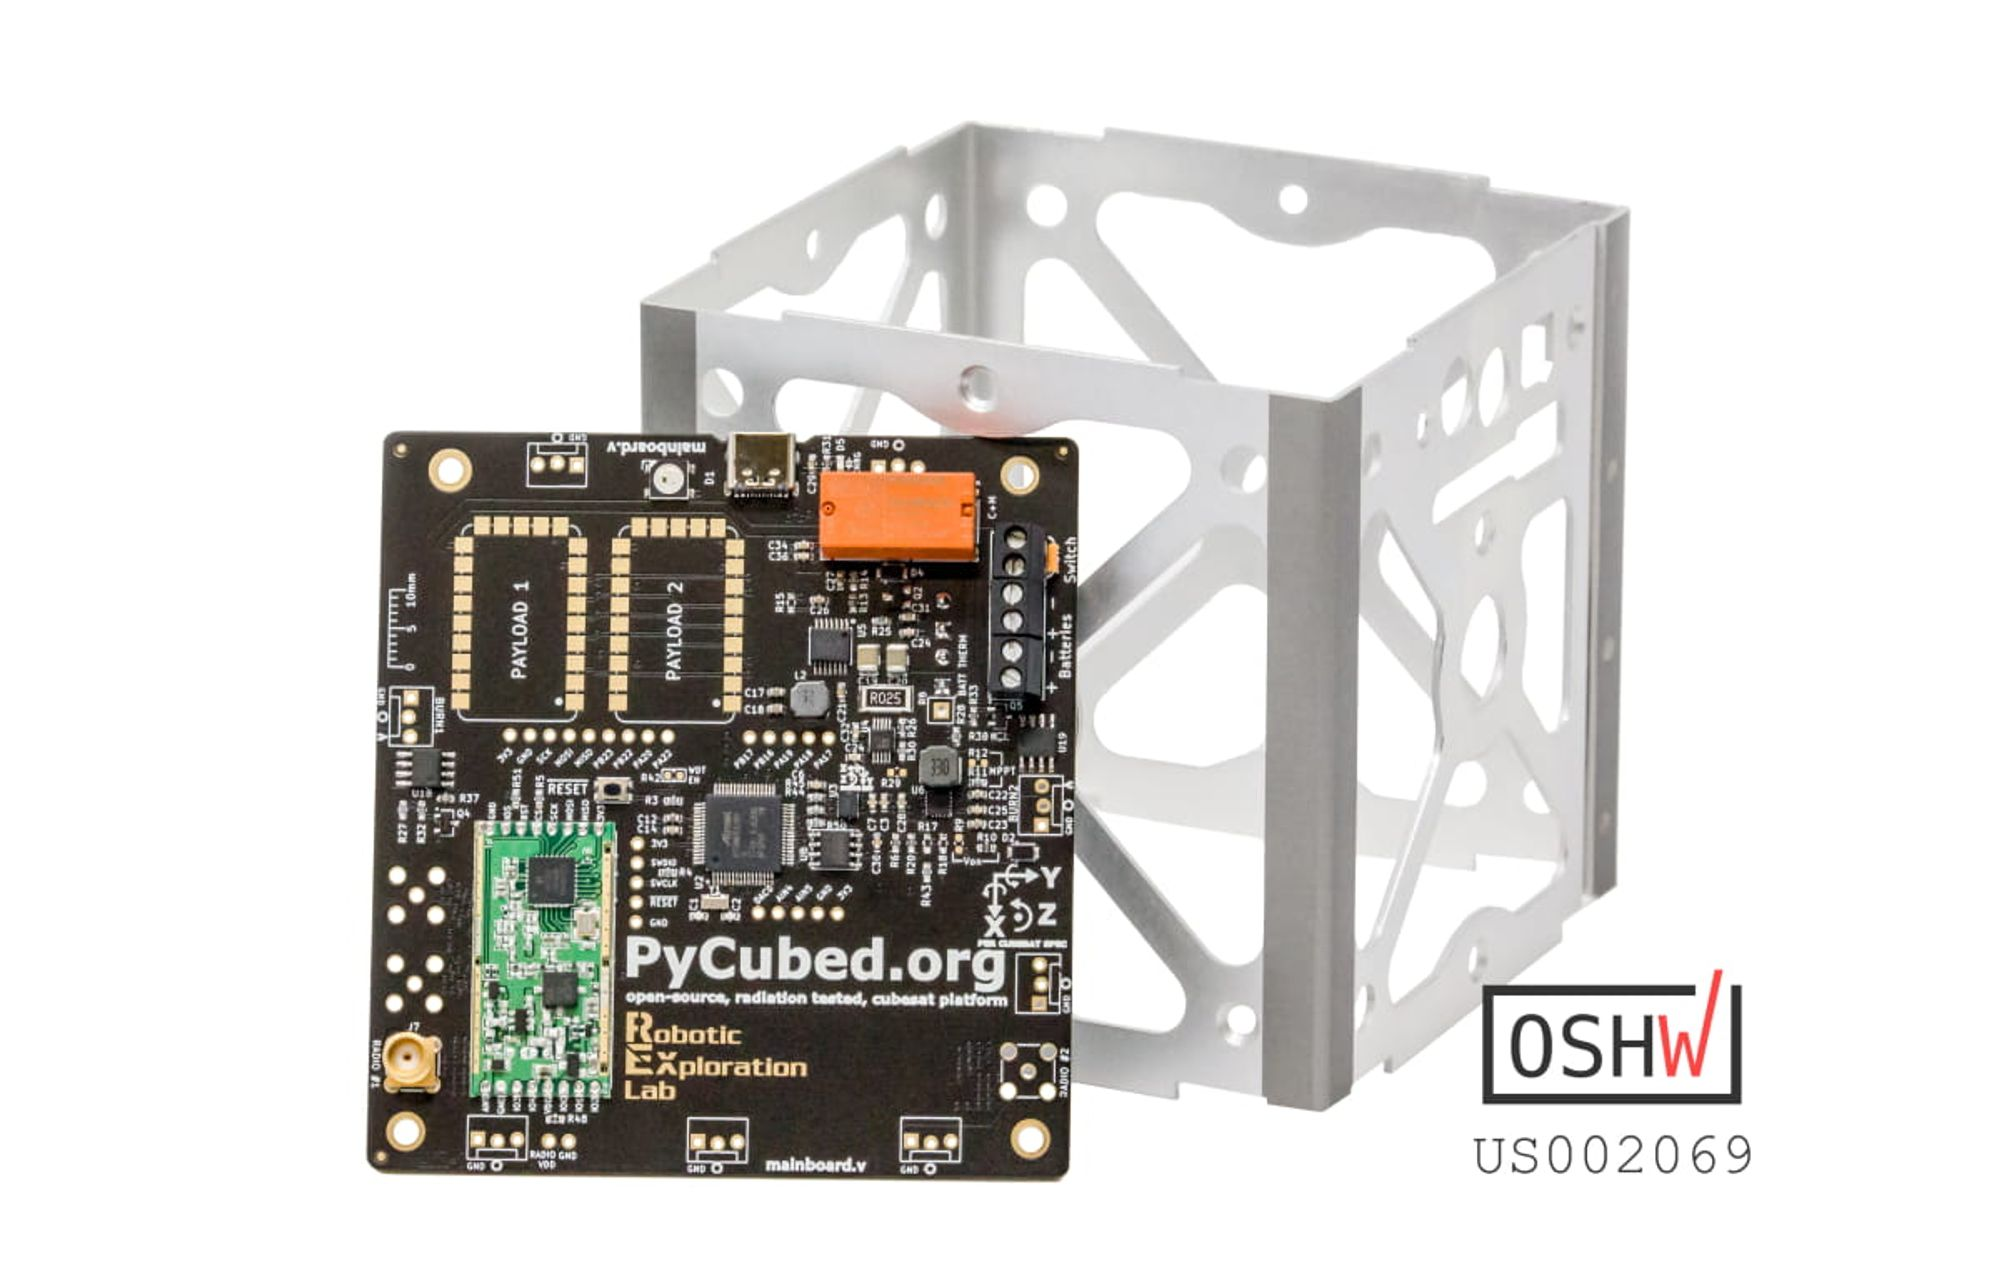
\includegraphics[width=0.75\textheight]{pycubed.jpg} % Reemplaza con tu primera imagen
            \mycaption{Proyecto Pycubed de la Universidad de Stanford \cite{pycubed}}
            \label{fig:sat3}
        \end{minipage}\hfill
        \begin{minipage}{.5\textwidth}
            \centering
            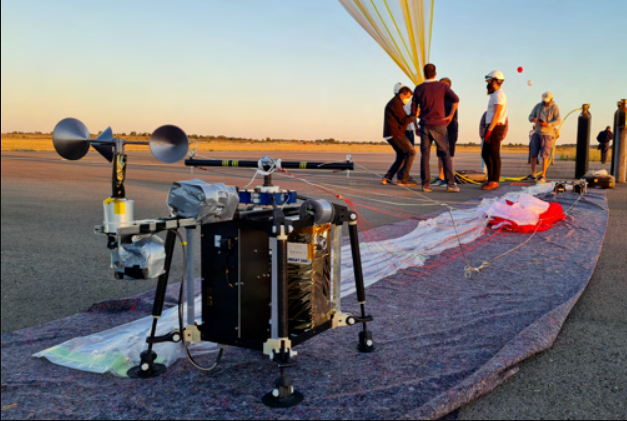
\includegraphics[width=.6\textheight]{TASEC_Lab.png} % Reemplaza con tu segunda imagen
            \vspace*{0.5 cm}
            \mycaption{Proyecto TASEC-Lab de la Universidad Politécnica de Madrid \cite{TASEC}}
            \label{fig:sat4}
        \end{minipage}
    \end{figure}    
    \end{frame}


% Página 4

\begin{frame}
    \frametitle{Anexo 3}
    \framesubtitle{Diseño: Relé, BJT, MOSFET}
    Se seleccionó un MOSFET, específicamente el modelo BS170, para el circuito de potencia, descartando relés debido a su alta disipación energética. Los MOSFET, siendo dispositivos de coeficiente térmico positivo (PTC) y controlados por voltaje, ofrecen una eficiencia superior a los BJT.
    \begin{figure}[H]
        \centering
        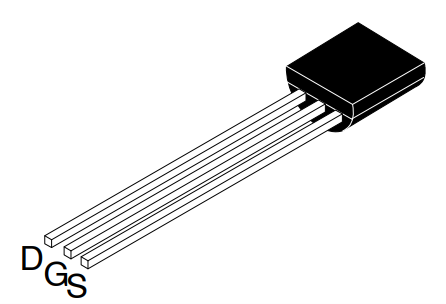
\includegraphics[width=0.4\textwidth]{BS170_Pinout.png} % Ajusta el tamaño según sea necesario
        \mycaption{MOSFET modelo BS170}
        \label{fig:BS170MOSFET}
    \end{figure}
    
    \end{frame}
    
    %PAGINA 5
    
    \begin{frame}
        \frametitle{Anexo 3}
        \framesubtitle{Diseño: Relé, BJT, MOSFET}
        \begin{figure}
            \centering
            \begin{minipage}{.5\textwidth}
                \centering
                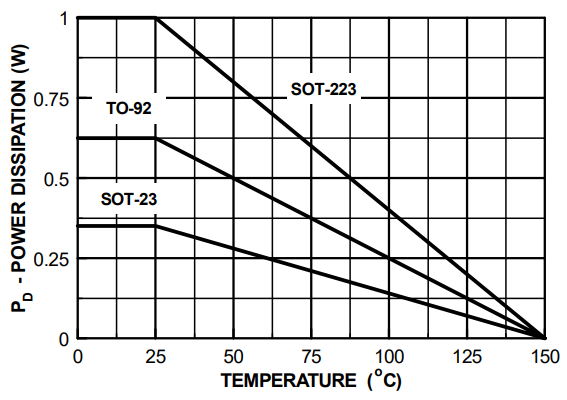
\includegraphics[width=0.65\textheight]{2N2222ApowerD.png} % Reemplaza con tu primera imagen
                \mycaption{Variación de potencia disipada en el 2N2222A en función de la
                temperatura ambiente}
                \label{fig:RESBJT}
            \end{minipage}\hfill
            \begin{minipage}{.5\textwidth}
                \centering
                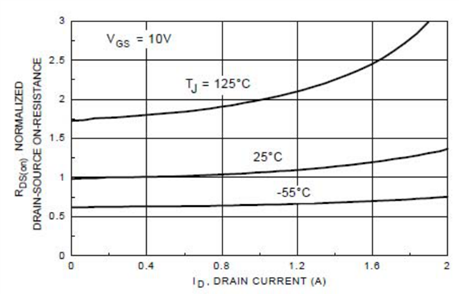
\includegraphics[width=.70\textheight]{resvscorriente.png} % Reemplaza con tu segunda imagen
                \mycaption{Variación de la resistencia interna en función de la corriente a distintas
                temperaturas ambiente.}
                \label{fig:RESMOSFET}
            \end{minipage}
        \end{figure}  
    \end{frame}
    

% Página 6 

\begin{frame}
    \frametitle{Anexo 4}
    \framesubtitle{Diseño: Simulación 4s1p, bus 3.3V}
    \begin{figure}[H]
        \centering
        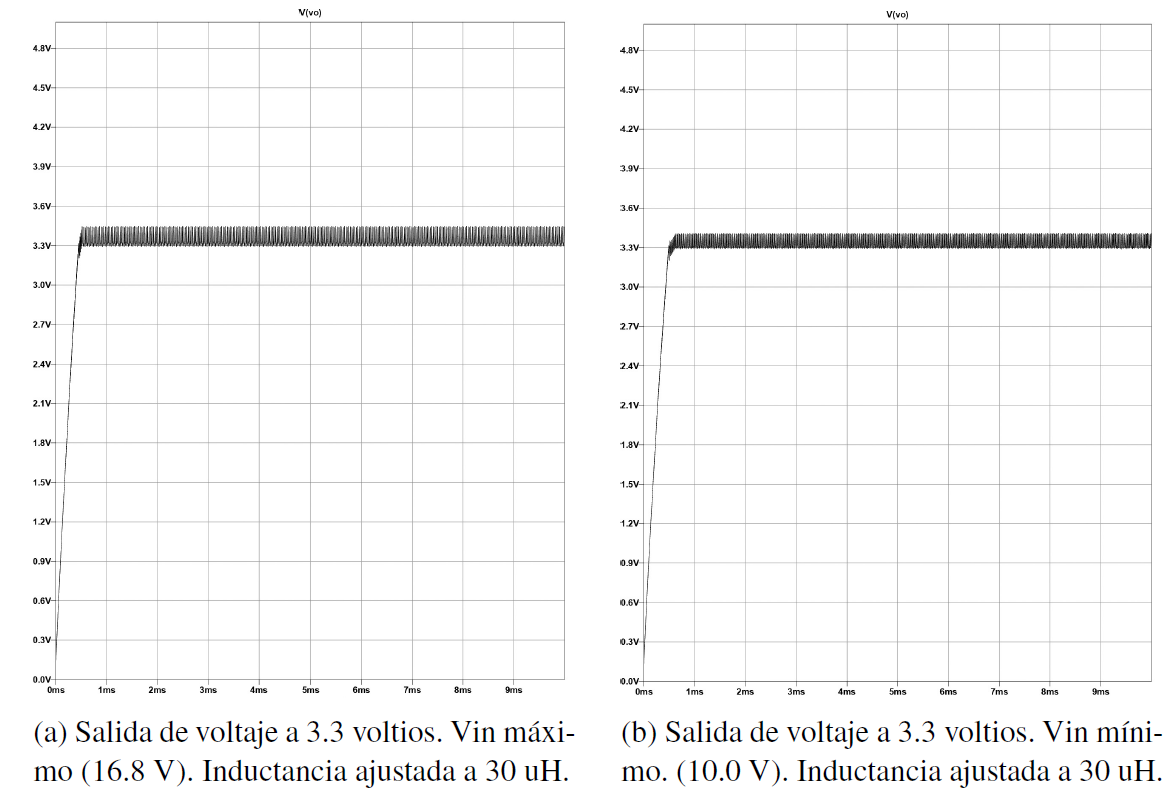
\includegraphics[width=0.7\textwidth]{4S1P_A.png} % Ajusta el tamaño según sea necesario
        \mycaption{Convertidor DC-DC MC34063A, arreglo 4s1p, bus de 3.3 V a 750 mA.}
        \label{fig:4S1P_A}
    \end{figure}
\end{frame}

%PAGINA 7
\begin{frame}
    \frametitle{Anexo 4}
    \framesubtitle{Diseño: Simulación 4s1p, bus 5.0V}
    \begin{figure}[H]
        \centering
        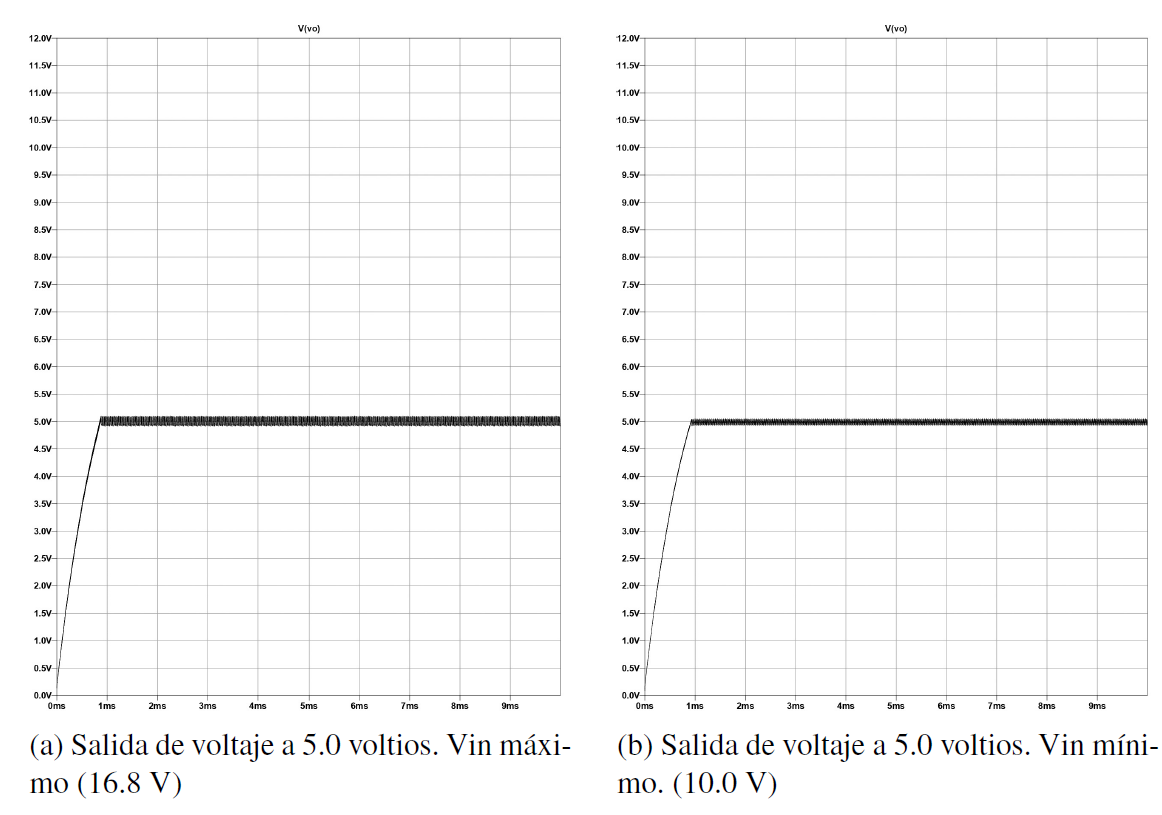
\includegraphics[width=0.7\textwidth]{4S1P_B.png} % Ajusta el tamaño según sea necesario
        \mycaption{Convertidor DC-DC MC34063A, arreglo 4s1p, bus de 5.0 V a 750 mA.}
        \label{fig:4S1P_B}
    \end{figure}
\end{frame}

%PAGINA 8
\begin{frame}
    \frametitle{Anexo 4}
    \framesubtitle{Diseño: Simulación 2s2p, bus 3.3V}
    \begin{figure}[H]
        \centering
        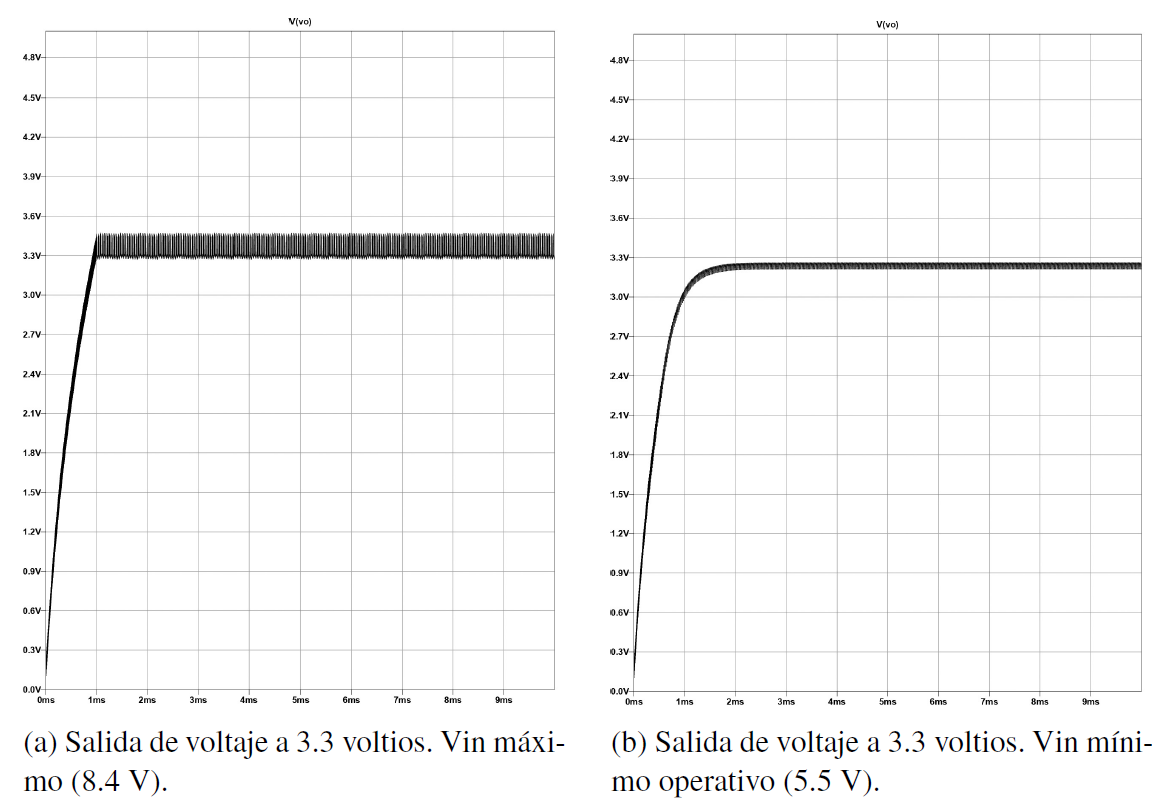
\includegraphics[width=0.7\textwidth]{2S2P_A.png} % Ajusta el tamaño según sea necesario
        \mycaption{Convertidor DC-DC MC34063A, arreglo 2s2p, bus de 3.3 V a 750 mA.}
        \label{fig:2S2P_A}
    \end{figure}
\end{frame}

%PAGINA 9
\begin{frame}
    \frametitle{Anexo 4}
    \framesubtitle{Diseño: Simulación 2s2p, bus 5.0V}
    \begin{figure}[H]
        \centering
        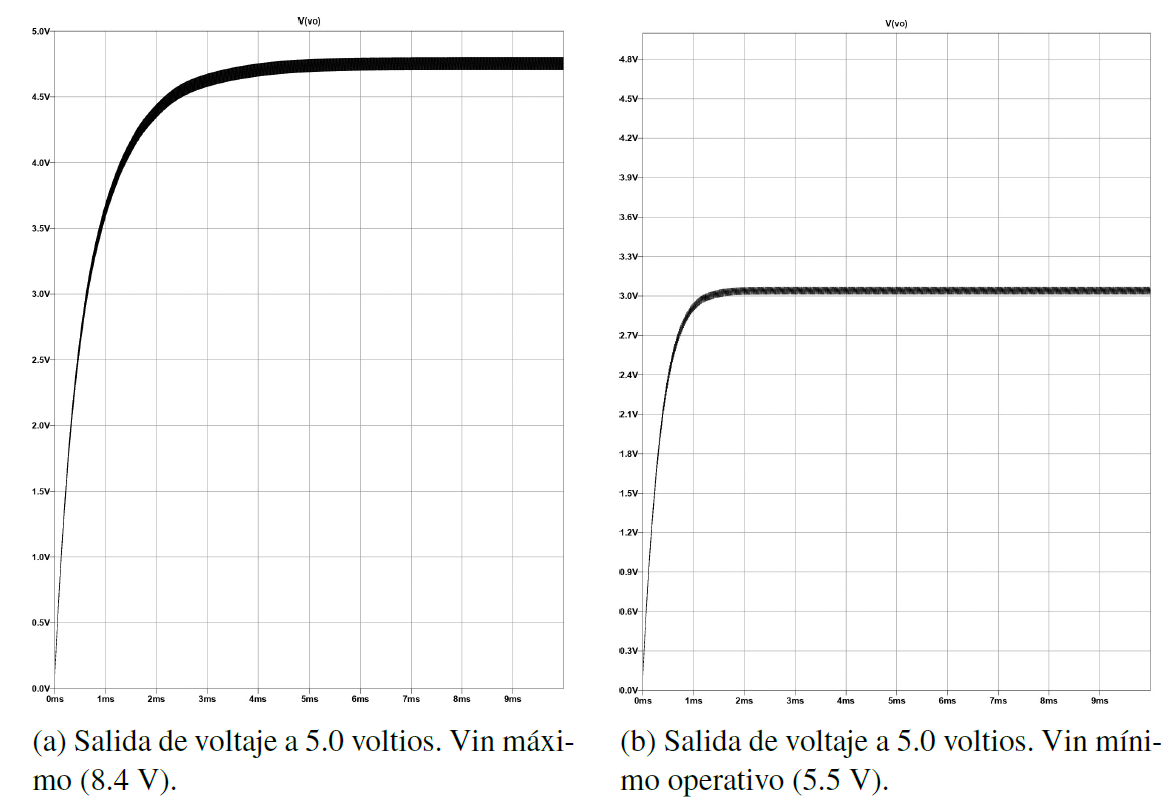
\includegraphics[width=0.7\textwidth]{2S2P_B.png} % Ajusta el tamaño según sea necesario
        \mycaption{Convertidor DC-DC MC34063A, arreglo 2s2p, bus de 5.0 V a 750 mA.}
        \label{fig:2S2P_B}
    \end{figure}
\end{frame}

%PAGINA 10

\begin{frame}
    \frametitle{Anexo 4}
    \framesubtitle{Diseño: Simulación 1s4p}
    
    La configuración 1s4p presenta un desafío: el voltaje de entrada al convertidor DC-DC a veces es mayor o menor que el voltaje de salida deseado. El MC34063A, que no ajusta automáticamente entre modos Buck y Boost, limita esta configuración.\\
    \vspace{0.5 cm}
    Futuras investigaciones podrían abordar esta limitación para aprovechar mejor el arreglo 1s4p. Dados los resultados, se ha elegido la configuración 4s1p para alcanzar de manera óptima los voltajes de salida requeridos de 3.3 V y 5.0 V.
\end{frame}

%Página 11

\begin{frame}
    \frametitle{Anexo 5}
    \framesubtitle{Integración del Sistema: Hardware}

    \begin{figure}[H]
        \centering
        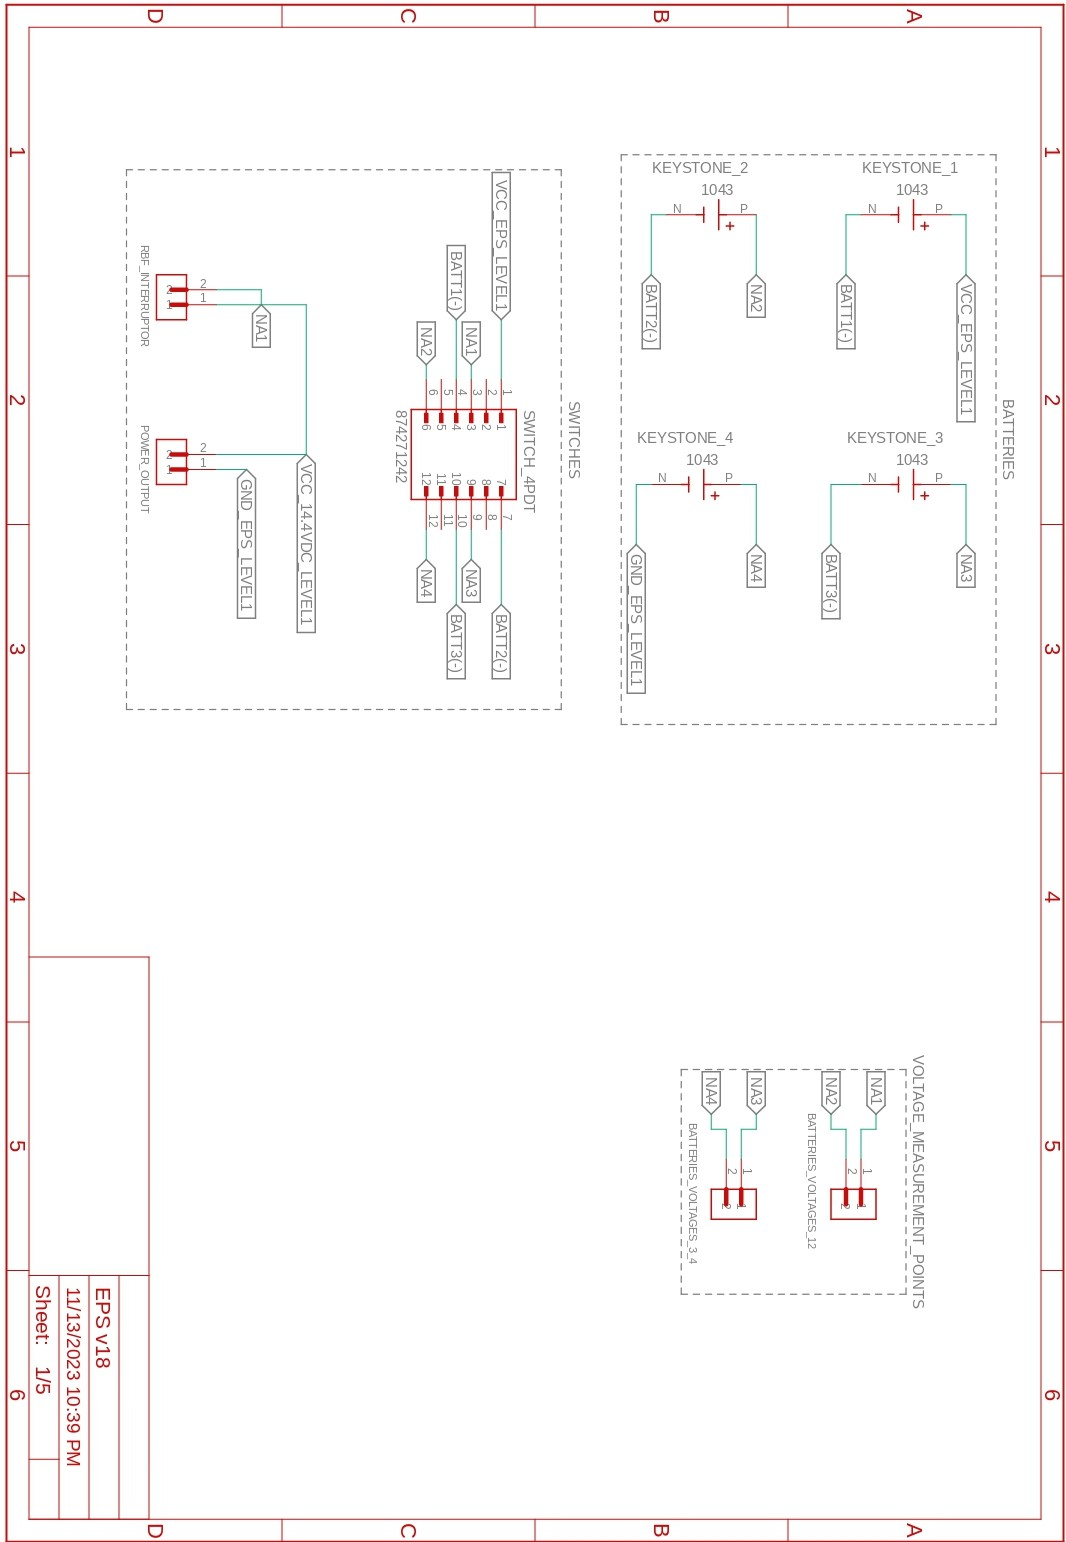
\includegraphics[width=0.6\textwidth, angle=90]{EPS_Sheets_page-0001.jpg} % Ajusta el tamaño y el ángulo según sea necesario
        \mycaption{Hoja 1 de esquemático del EPS}
        \label{fig:Esquematico1}
    \end{figure}
\end{frame}


%PAGINA 12

\begin{frame}
    \frametitle{Anexo 5}
    \framesubtitle{Integración del Sistema: Hardware}
    \begin{figure}[H]
        \centering
        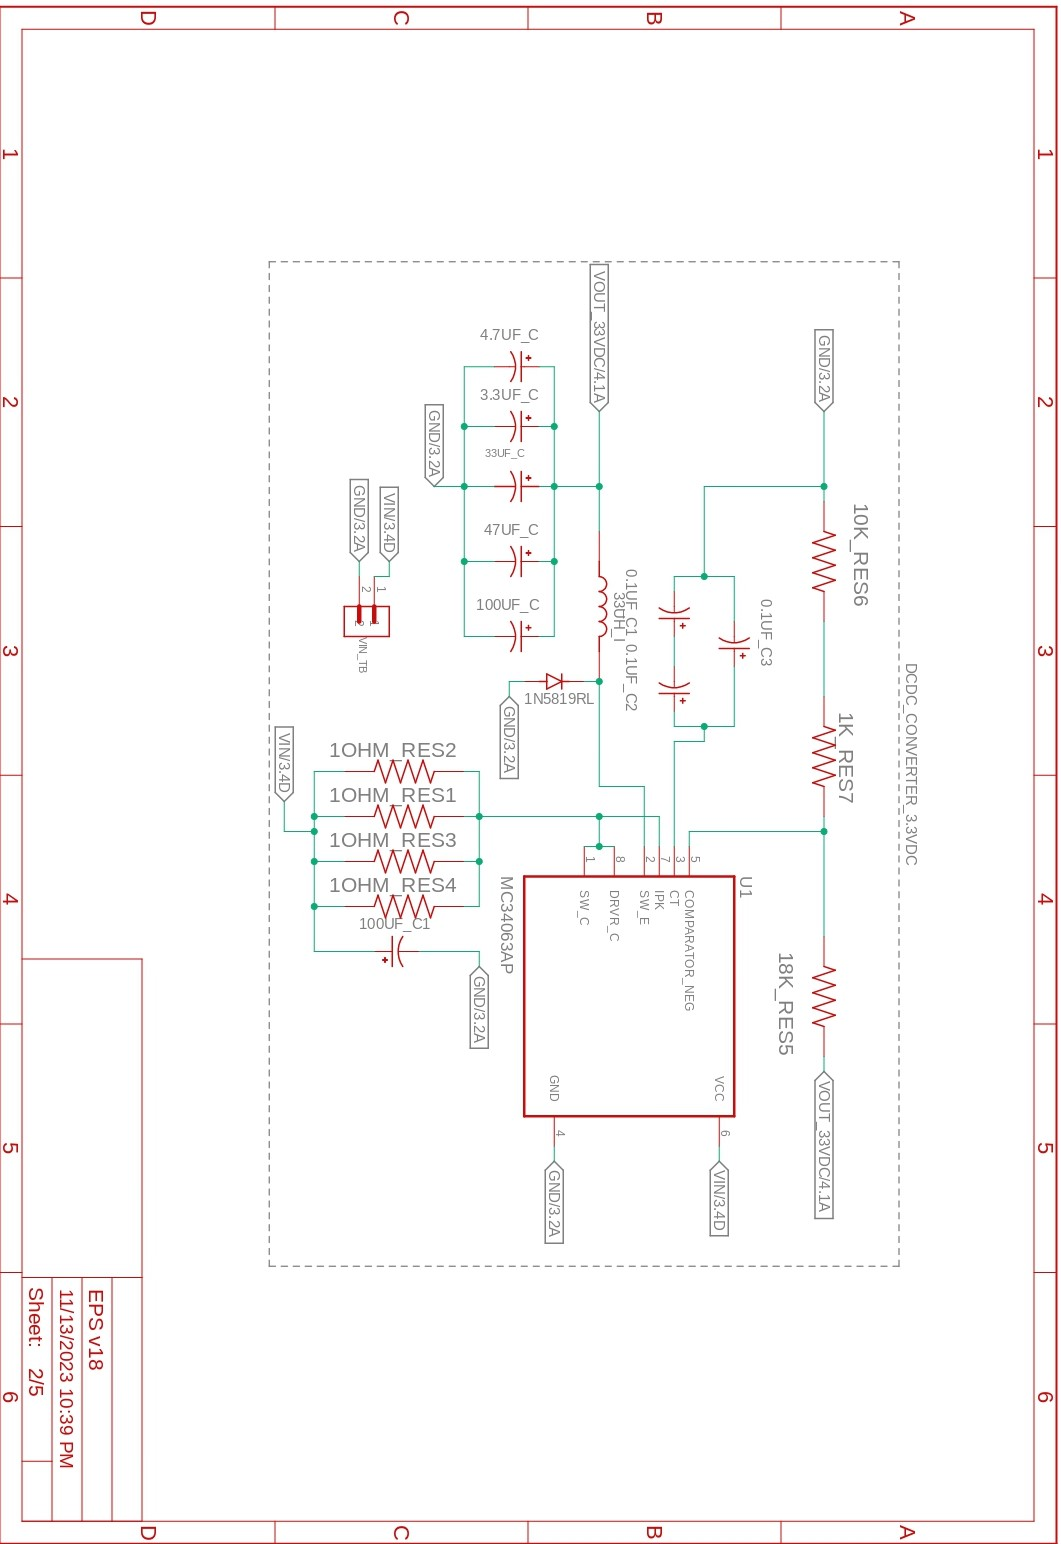
\includegraphics[width=0.6\textwidth, angle=90]{EPS_Sheets_page-0002.jpg} % Ajusta el tamaño según sea necesario
        \mycaption{Hoja 2 de esquemático del EPS}
        \label{fig:Esquematico2}
    \end{figure}
\end{frame}

%PAGINA 13

\begin{frame}
    \frametitle{Anexo 5}
    \framesubtitle{Integración del Sistema: Hardware}
    \begin{figure}[H]
        \centering
        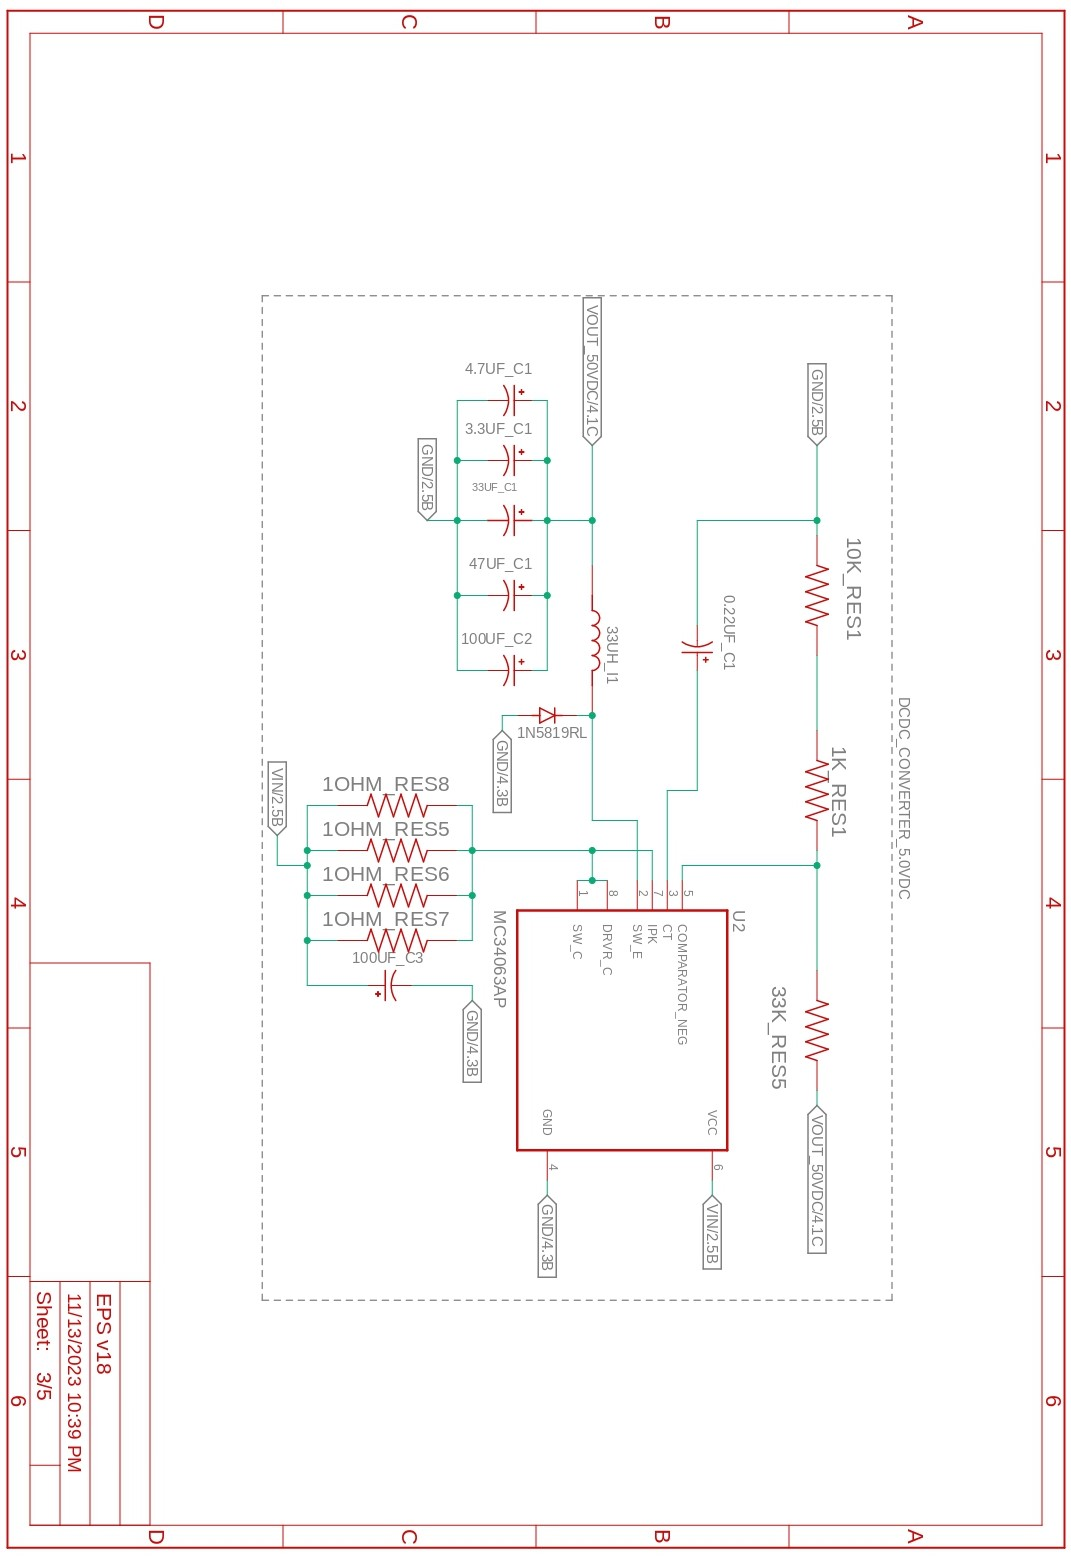
\includegraphics[width=0.6\textwidth, angle=90]{EPS_Sheets_page-0003.jpg} % Ajusta el tamaño según sea necesario
        \mycaption{Hoja 3 de esquemático del EPS}
        \label{fig:Esquematico4}
    \end{figure}
\end{frame}

%PAGINA 14

\begin{frame}
    \frametitle{Anexo 5}
    \framesubtitle{Integración del Sistema: Hardware}
    \begin{figure}[H]
        \centering
        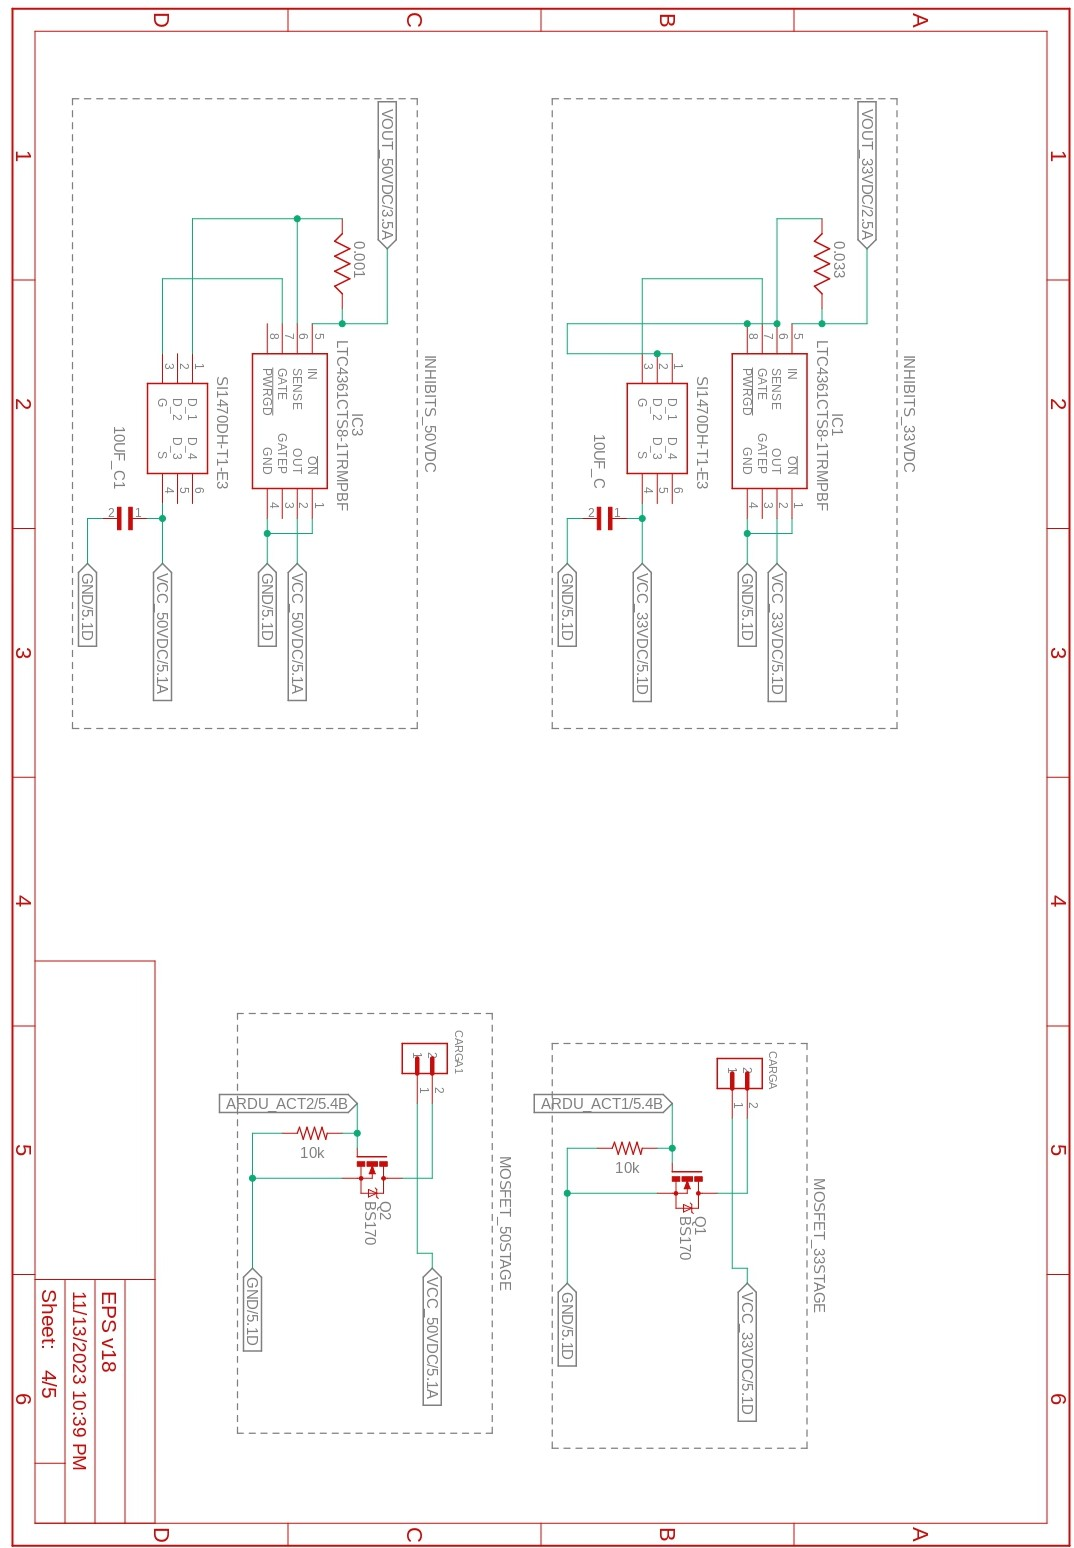
\includegraphics[width=0.6\textwidth, angle=90]{EPS_Sheets_page-0004.jpg} % Ajusta el tamaño según sea necesario
        \mycaption{Hoja 4 de esquemático del EPS}
        \label{fig:Esquematico4}
    \end{figure}
\end{frame}

%PAGINA 15

\begin{frame}
    \frametitle{Anexo 5}
    \framesubtitle{Integración del Sistema: Hardware}
    \begin{figure}[H]
        \centering
        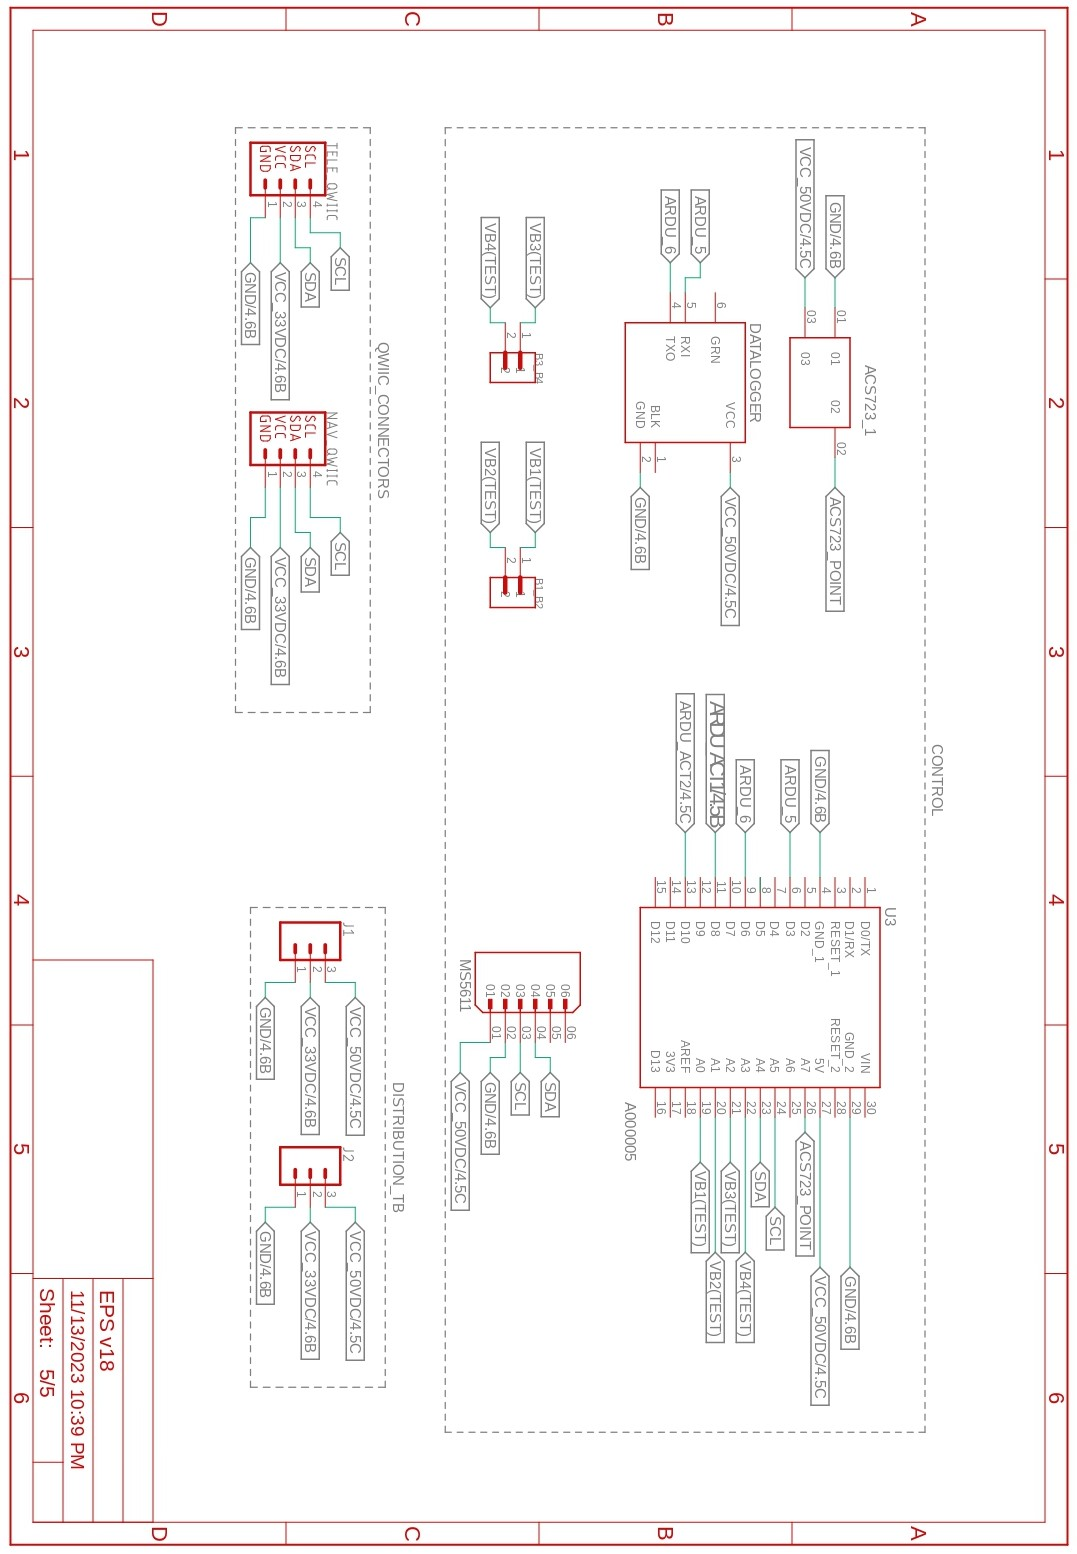
\includegraphics[width=0.6\textwidth, angle=90]{EPS_Sheets_page-0005.jpg} % Ajusta el tamaño según sea necesario
        \mycaption{Hoja 5 de esquemático del EPS}
        \label{fig:Esquematico5}
    \end{figure}
\end{frame}

%PAGINA 16

\begin{frame}
    \frametitle{Anexo 6}
    \framesubtitle{Contribuciones de la Tesis}
    \begin{itemize}
        \item Aplicación de Metodología de la NASA: Adaptación y aplicación en el diseño y desarrollo de un EPS para HAB.
        \item Desarrollo Integral del EPS: Incluye documentación detallada sobre desarrollo con software libre y electrónica COTS.
        \item Caracterización ambiental a lo largo de la trayectoria de un HAB: análisis del comportamiento de variables ambientales, como temperatura y presión, basado en datos provenientes de simulaciones de la trayectoria. Véase el Anexo B del documento de la Tesis.
    \end{itemize}
    
    
\end{frame}

%PAGINA 17

\begin{frame}
    \frametitle{Anexo 7}
    \framesubtitle{Trabajos Futuros}
    \begin{itemize}
        \item Cargador de baterías a bordo.
        \item Cámara de Vacío Térmico de Bajo Costo.
        \item Convertidor DC-DC para Arreglo de Baterías 1s4p.
        \item Diseño de Circuito de Descarga a Corriente Constante para Baterías de
        Iones de Litio.
    \end{itemize}
    
\end{frame}

%PAGINA 18

\begin{frame}
    \frametitle{Anexo 8}
    \framesubtitle{Presupuesto: EPS}
 
    \begin{table}[!ht]
        \centering
        \begin{tabular}{ll}
        \hline
            \textbf{\hfill Presupuesto de Compras \hfill} &  \\ \hline
            Local & \$64.59 \\ 
            Internacional & \$220.696 \\ 
            \hline
            Total & \$285.286 \\ 
        \hline
        \end{tabular}
        \caption{Resumen del Presupuesto de Compras}
        \label{tab:presupuesto}
    \end{table}
    
    
\end{frame}

